%%%%%%%%%%%%%%%%%%%%%%%%%%%%%%%%%%%%%%%%%
% Journal Article
% LaTeX Template
% Version 1.4 (15/5/16)
%
% This template has been downloaded from:
% http://www.LaTeXTemplates.com
%
% Original author:
% Frits Wenneker (http://www.howtotex.com) with extensive modifications by
% Vel (vel@LaTeXTemplates.com)
%
% License:
% CC BY-NC-SA 3.0 (http://creativecommons.org/licenses/by-nc-sa/3.0/)
%
%%%%%%%%%%%%%%%%%%%%%%%%%%%%%%%%%%%%%%%%%

%----------------------------------------------------------------------------------------
%	PACKAGES AND OTHER DOCUMENT CONFIGURATIONS
%----------------------------------------------------------------------------------------

\documentclass[twoside,twocolumn]{article}

\usepackage{blindtext} % Package to generate dummy text throughout this template 

\usepackage[sc]{mathpazo} % Use the Palatino font
\usepackage[T1]{fontenc} % Use 8-bit encoding that has 256 glyphs
\linespread{1.05} % Line spacing - Palatino needs more space between lines
\usepackage{microtype} % Slightly tweak font spacing for aesthetics

\usepackage[english]{babel} % Language hyphenation and typographical rules

\usepackage[hmarginratio=1:1,top=32mm,columnsep=20pt]{geometry} % Document margins
\usepackage[hang, small,labelfont=bf,up,textfont=it,up]{caption} % Custom captions under/above floats in tables or figures
\usepackage{booktabs} % Horizontal rules in tables

\usepackage{lettrine} % The lettrine is the first enlarged letter at the beginning of the text

\usepackage{enumitem} % Customized lists
\setlist[itemize]{noitemsep} % Make itemize lists more compact

\usepackage{abstract} % Allows abstract customization
\renewcommand{\abstractnamefont}{\normalfont\bfseries} % Set the "Abstract" text to bold
\renewcommand{\abstracttextfont}{\normalfont\small\itshape} % Set the abstract itself to small italic text

\usepackage{titlesec} % Allows customization of titles
\renewcommand\thesection{\Roman{section}} % Roman numerals for the sections
\renewcommand\thesubsection{\roman{subsection}} % roman numerals for subsections
\titleformat{\section}[block]{\large\scshape\centering}{\thesection.}{1em}{} % Change the look of the section titles
\titleformat{\subsection}[block]{\large}{\thesubsection.}{1em}{} % Change the look of the section titles

\usepackage{fancyhdr} % Headers and footers
\pagestyle{fancy} % All pages have headers and footers
\fancyhead{} % Blank out the default header
\fancyfoot{} % Blank out the default footer
\fancyhead[C]{5584F $\bullet$ March 2020 $\bullet$ 4G3} % Custom header text
\fancyfoot[RO,LE]{\thepage} % Custom footer text

\usepackage{titling} % Customizing the title section

\usepackage{hyperref} % For hyperlinks in the PDF

\usepackage{graphicx}
\graphicspath{ {images/} }

\newenvironment{reusefigure}[2][htbp]
  {\addtocounter{figure}{-1}%
   \renewcommand{\theHfigure}{dupe-fig}% If you're using hyperref
   \renewcommand{\thefigure}{\ref{#2}}% Figure counter is \ref
   \renewcommand{\addcontentsline}[3]{}% Avoid placing figure in LoF
   \begin{figure}[#1]}
  {\end{figure}}
\usepackage{wrapfig}
\usepackage{wrapfig}
\usepackage{amsmath}
\usepackage{xcolor}
\usepackage{listings}
\usepackage{subcaption}
\usepackage{pdfpages}
\usepackage{array,multirow,graphicx}
\lstset{
  basicstyle=\ttfamily,
  columns=fullflexible,
  frame=single,
  breaklines=true,
  postbreak=\mbox{\textcolor{red}{$\hookrightarrow$}\space},
}

\newcommand{\threepartdef}[6]
{
	\left\{
		\begin{array}{lll}
			#1 & \mbox{: } #2 \\
			#3 & \mbox{: } #4 \\
			#5 & \mbox{: } #6 \\
			0 & \mbox{: } otherwise
		\end{array}
	\right.
}
%----------------------------------------------------------------------------------------
%	TITLE SECTION
%----------------------------------------------------------------------------------------

\setlength{\droptitle}{-4\baselineskip} % Move the title up

\pretitle{\begin{center}\Huge\bfseries} % Article title formatting
\posttitle{\end{center}} % Article title closing formatting
\title{4G3 - Coursework Two -  Hopfield network and spiking neurons} % Article title
\author{%
\\
\textsc{Candidate Number: 5584F} \\
}
\date{\today} % Leave empty to omit a date
\renewcommand{\maketitlehookd}{%
\begin{abstract}
\noindent
Hopfield networks and firing using the Hodgkin-Huxley model were investigated. In a Hopfield network partial memories can be retrieved as stored memories act as attractors for convergence on average. Errors can occur in retrieval of noisy memories as other attractors e.g inverted memories are converged upon. The Hodgkin-Huxley model includes the effect of different ion channels on membrane currents and potentials. This extra complexity allows the modelling of behaviours that oscillate in different limit cycles, respond to resonant frequencies and have sharp input thresholds to induce firing. 
\newline
\end{abstract}
}

%----------------------------------------------------------------------------------------

\begin{document}
\onecolumn
\includepdf[pages={1}]{Coversheet.pdf}
\twocolumn
\pagenumbering{arabic}
% Print the title
\maketitle
%----------------------------------------------------------------------------------------
%	ARTICLE CONTENTS
%----------------------------------------------------------------------------------------
\section{Introduction}

\lettrine[nindent=0em,lines=3]{A}ssociative memory is the process of retrieving a memory from partial data. This is to be investigated using a Hopfield network, to consider the effect of noise and instability within the network.
\newline
A physiologically realistic model of a spiking neuron was then investigated using the Hodgkin-Huxley model to discover the differences from more simplistic models such as leaky integrate and fire neurons. 

%------------------------------------------------

\section{Hopfield network}
A binary Hopfield network was investigated. This network is fully connected with each neuron having an activity of 0 or 1. This network can be used to store binary strings (memories), which are retrievable with partial information about the memory. This retrieval is possible as the network weights are chosen as in equation \ref{eq:weights}, this choice causes memories to be stable fixed points on average and thus can be converged upon. The success of this convergence was analysed.

%------------------------------------------------
\subsection{ Theoretical error probability}
\begin{figure}[h]
  \centering
    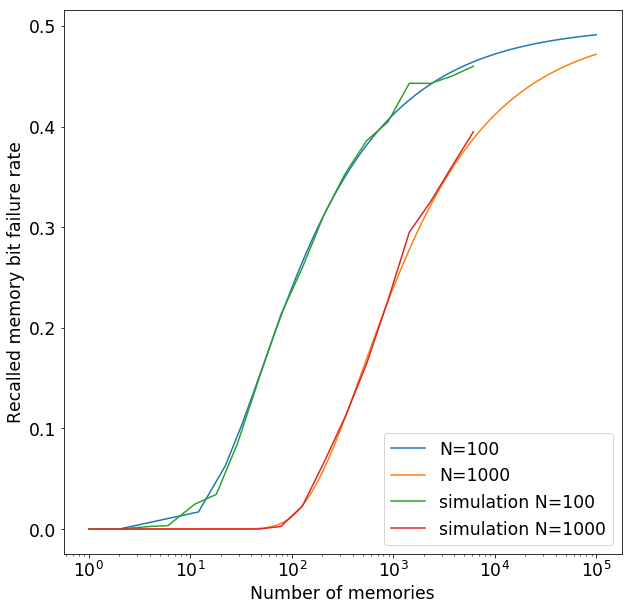
\includegraphics[width=\linewidth]{1a}
  \caption{Simulations one step}
  \label{sub:ep1}
\end{figure}

\begin{figure}[h]
  \centering
    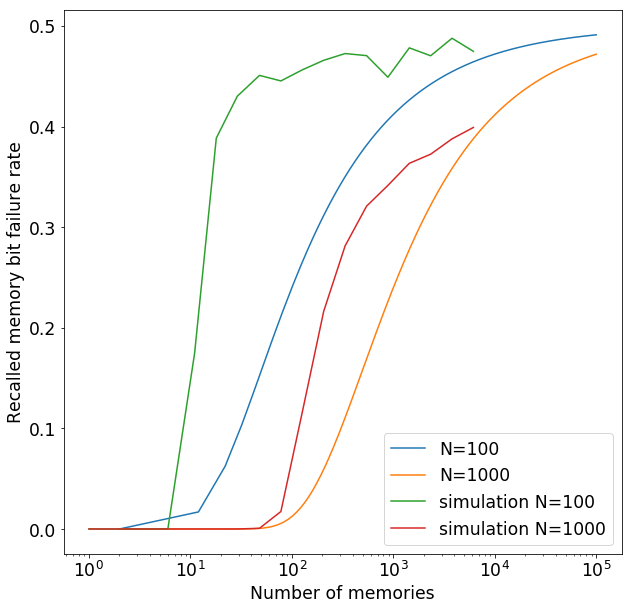
\includegraphics[width=\linewidth]{1}
  \caption{Simulations 3000 step}
  \label{sub:ep3000}
\end{figure}



Errors during memory recall can occur from: 
\begin{itemize}
\item Points that are not memories act as attractors and cause convergence, these spurious attractors take the form of combinations of stored memories or inverted memories
\item Stored memories are unstable, and therefore with a disturbance the retrieval will drift or oscillate
\item Stored memories are not fixed points therefore convergence to them doesn't occur
\end{itemize}
Within the space of dimension N exists the local field on each bit $H_k = \sum_{j\neq k} W_{kj}r_j(t)$ this is prevalent in the update term in equation \ref{eq:update}. This field is constructed as in equation \ref{eq:weights} such that the field points towards stored memories on average. This helps the retrieval of partial memories. The field can be broken down into two terms:

\begin{gather}
H_k = (r_k^{(\mu)}-\frac{1}{2})\sum\limits_{j \neq k} r_j^{(\mu)}(r_j^{(\mu)}-\frac{1}{2}) \nonumber \\
+\sum\limits_{j \neq k} r_j^{(\mu)} \sum\limits_{m \neq \mu}(  (r_j^{(m)}-\frac{1}{2})(r_k^{(m)}-\frac{1}{2})  \nonumber
\end{gather}

With the first term being the contribution from the desired memory $\mu$ and the second the contribution from all other stored memories and is classed as noise. The two terms have the following mean and variance, given the desired memory and with each state equally probable:

\begin{align}
<signal> =& \pm \frac{N-1}{8} \nonumber \\
<noise> =& 0 \nonumber \\
<<signal>> =& 0 \nonumber\\
<<noise>> =& \frac{(N-1)(M-1)}{32} \nonumber 
\end{align}

On average the noise terms are zero which means that memory states are on average a stable fixed point. However, if the noise term is larger then the signal mean, and resides in the correct tail the local field can point the wrong direction. This means that memory is not a fixed point. This error can be theoretically computed as P($H_k<0|r_k^{(\mu)}=1)$, where $H_k \sim \mathcal{G}(\frac{N-1}{8},\frac{(N-1)(M-1)}{32}$). $H_k$ is Gaussian as its the sum of many random variables so is Gaussian by the CLT. The error as a function of stored memories is shown in figure \ref{sub:ep1}.
\newline
As the number of memories stored increases, memories and attractors become closer within the space ($\mathcal{R}^N$). This increases the weight of each attractor on a memory being retrieved and therefore increases the noise prevalent in convergence. This additional noise increases the error probability.
\newline
The calculated probability is conditional on the memory being the starting point, and then checking the field. The probability of a state being fixed but not stable is not considered. This probability will effect error rates when noise or full convergence is simulated.
%\newline
%To include the effect from unstable memories an %additional error term would need to be added which %induces the probability a memory is unstable as a %function of M,N. As these memories would be greater %effected by noise, and need to be treated differently.
%------------------------------------------------
\subsection{ Simulations}
To create a network that converges upon memories in the desired way connectivity weights are chosen as in equation \ref{eq:weights}. When recalling a memory at each iteration a single neuron is asynchronously updated using equation \ref{eq:update}. These updates can be repeated until convergence.

\begin{equation}
W_{ij} =
\left\{
	\begin{array}{ll}
		\sum\limits^M_{m=1}(r_i^{(m)}-\frac{1}{2})(r_j^{(m)}-\frac{1}{2})  &  i \neq j \\
		0 & i=j
	\end{array}
\right.
\label{eq:weights}
\end{equation}

\begin{equation}
r_i(t+\Delta t)=\frac{sign[\sum\limits_{j=1}^NW_{ij}r_j(t)]+1}{2}
\label{eq:update}
\end{equation}
When simulating network convergence you can't isolate one type of error as additional update steps have a chance of causing error from one of the three methods. This means that the bit error calculated will include differences caused by unstable/oscillatory memories in addition to non-fixed point memories as theoretically calculated. Errors caused in one bit can effect later update steps and cause more errors.
However, if you simulate just one step then check if the memory has been recalled correctly you are testing on average if a bit converges correctly therefore checking fixed points. Figure \ref{sub:ep1} shows the results of this simulation for N=100 and 1000, averaged over 100 networks. This result is shown to agree very closely to the theoretical error term calculated above.
\newline
When recalling memories convergence is required to properly test recall ability.
If the network is ran for 3000 steps to allow for convergence to occur the results in figure \ref{sub:ep3000} are produced. This produces a steeper curve then the predicted error probability as spurious attractors and unstable/oscillatory memory states have a greater effect. This bit error rate is more useful to consider when calculating network capacities.

%------------------------------------------------
\subsection{Noise}
\begin{figure}[h]
  \centering
    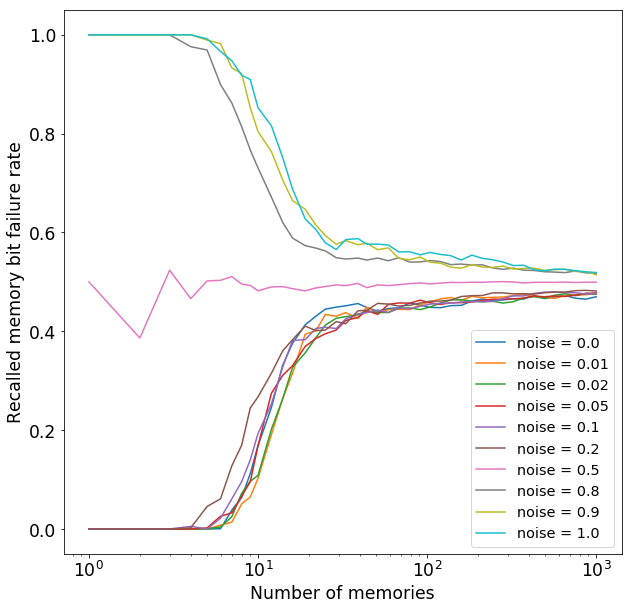
\includegraphics[width=\linewidth]{noise2}
  \caption{Simulations with varying noise levels}
  \label{fig:noise}
\end{figure}

Figure \ref{fig:noise} shows the results from simulating 10 Hopfield networks for 3000 steps to allow for convergence, and calculating the average probability of a bit being incorrectly recalled from a noisy memory. The noisy memory is made by flipping each bit in a memory by a certain probability. 
\newline
The results show that noise levels below 0.2 result in similar curves to a noiseless case, with levels above 0.8 being the same but mirrored in y=0.5. At a noise level of 0.5 the recall rate is quite noisy but can be seen to be a constant 0.5, independent of M. This shows that convergence is happening to random memories and not the initial memory. 
\newline
All curves converge upon a failure rate of 0.5 as the number of stored memories increases. This is due to the space ($\mathcal{R}^N$) becoming very crowded, meaning small changes due to noise cause corrupted memories to converge upon different memories or spurious attractors, and therefore have 50\% of bits different on average.
\newline
At a noise level above 0.5 the memory gets changed to be closer to its inverted memory. In a Hopfield network inverted stored memory are also attractors, this means that when retrieving the memory the attraction from the inverted memory is stronger then the true memory. Therefore convergence occurs to that and the bit failure rate is close to or equal 1.
\newline
Surprisingly when noise was 0 the network didn't perform the best. This would be expected as unstable fixed point memories would be greatly effected by the introduction of noise. Therefore causing greater bit errors. This difference could be explained due to insufficient averaging across networks, and the inherent randomness in testing.
 %----------------------------------------------- 
 \newpage
\section{Physiological model of a spiking neuron}
To build a physiological model of spiking neurons different channels into a neuron must be considered. In these experiments the Hodgkin Huxley model of action potentials will be investigated. This model includes channels for a leakage current (L), potassium ions (K) and sodium ions (Na). These channels have maximum conductance densities and reversal potentials associated with them defined by $g_x,e_x$ respectively. The sodium and potassium channel conductances are functions of both time and voltage, and therefore require the additional m, h,  and n terms. These terms are sodium channel activation, sodium channel deactivation and potassium channel activation respectively and are controlled by $\alpha$ and $\beta$ functions. This model could be extended to include additional ion channels. Equations \ref{eq:integration} define the forward euler update steps used during simulations.
\begin{figure}[h]
  \centering
    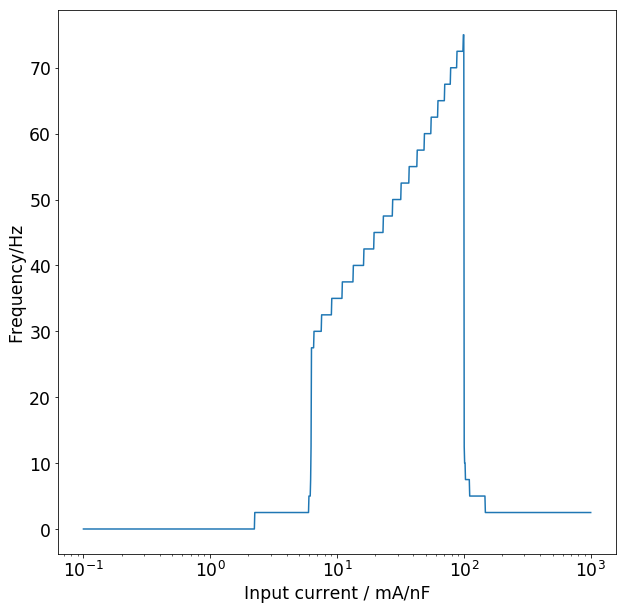
\includegraphics[width=0.85\linewidth]{fl}
  \caption{Response to 200ms pulse, 400ms period input}
  \label{fig:2aw}
\end{figure}

\begin{equation}
\begin{split}
v_{t+\Delta t} = ( -g_{Na}.m_t^3 h_t(v_t-e_{Na})  -g_K.n_t^4(v_t-e_K)  \\ -g_L(v_t-e_L) + I)\Delta t + v_t \\
m_{t+\Delta t} =  ( \alpha_m(v_t)(1-m_t) - \beta_m(v_t)m_t ) \Delta t + m_t \\
   h_{t+\Delta t}  =  ( \alpha_h(v_t)(1-h_t) - \beta_h(v_t)h_t ) \Delta t + h_t \\
    n_{t+\Delta t}  =  ( \alpha_n(v_t)(1-n_t) - \beta_n(v_t)n_t )\Delta t + n_t \\
\end{split}
\label{eq:integration}
\end{equation}

%------------------------------------------------
\subsection{ Constant pulse}





\begin{figure}[h]
  \centering
    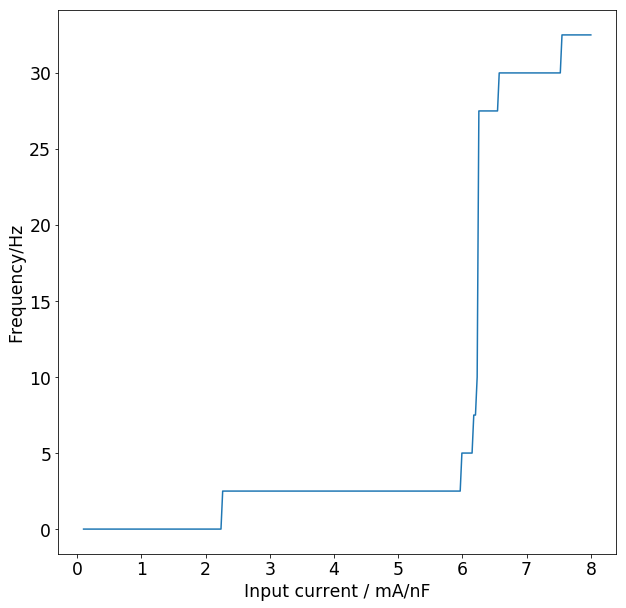
\includegraphics[width=\linewidth]{fd1}
  \caption{Response to 200ms pulse, 400ms period input at low currents}
  \label{fig:2al}
\end{figure}


The external input I was varied from 0.1mA/nF - 1A/nF for pulse of length 200ms, and period 400ms. Figure \ref{fig:2aw} shows the firing frequency as a function of this input. A sharp threshold is observed for continuous firing to occur. This happens between 6.11-6.26mA/nF. This is an example of an all or none response to the input. The firing rate increases approximately logarithmically in steps until an input around 100mA/nF upon which the response follows the pulse shape with very small oscillations and one spike as in figure \ref{sub:2a150}. Example responses can be seen before the firing threshold in figures \ref{sub:2a0-1} and  \ref{sub:2a1-6}, with 0.1mA/nF causing almost no change, and 1.6mA/nF causing small disturbances from the rest potential/current. With an input of 2.5mA/nF as in figure \ref{sub:2a2-5} single spikes are observed in membrane potentials and currents. A double spike is briefly possible at 6.11mA/nF (\ref{sub:2a6-11}) before continuous firing is reached at 6.26mA/nF (\ref{sub:2a6-26}). During continuous firing, spikes occur at regular intervals, this is due to the limit cycle prevalent in the model, which causes regular oscillations.

\onecolumn

\begin{figure}[h]
  \centering
  \begin{subfigure}[t]{0.49\textwidth}
    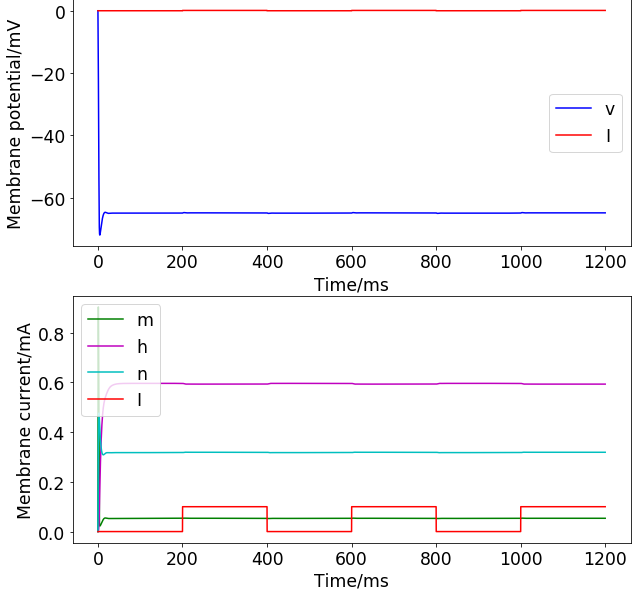
\includegraphics[width=\linewidth]{a0-1}
  \caption{0.1mA/nF}
  \label{sub:2a0-1}
  \end{subfigure}
  \begin{subfigure}[t]{0.49\textwidth}
    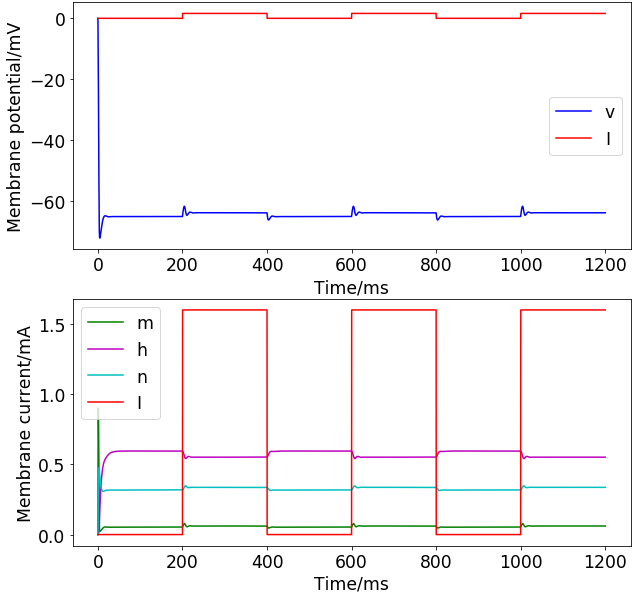
\includegraphics[width=\linewidth]{a1-6}
  \caption{1.6mA/nF}
  \label{sub:2a1-6}
  \end{subfigure}
\newline
  \begin{subfigure}[t]{0.49\textwidth}
    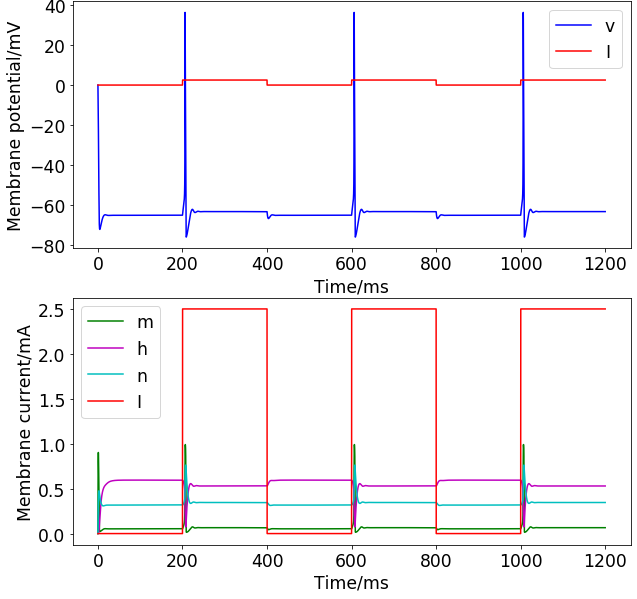
\includegraphics[width=\linewidth]{a2-5}
  \caption{2.5mA/nF}
  \label{sub:2a2-5}
  \end{subfigure}
  \begin{subfigure}[t]{0.49\textwidth}
    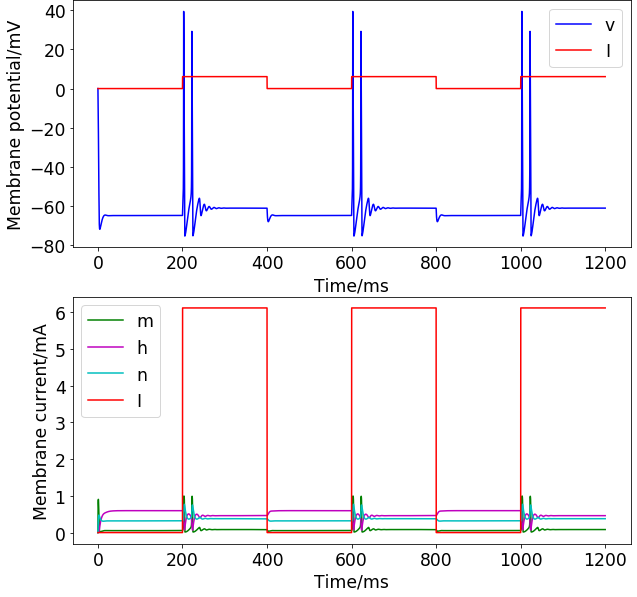
\includegraphics[width=\linewidth]{a6-11}
  \caption{6.11mA/nF}
  \label{sub:2a6-11}
  \end{subfigure}
\newline
\begin{subfigure}[t]{0.49\textwidth}
    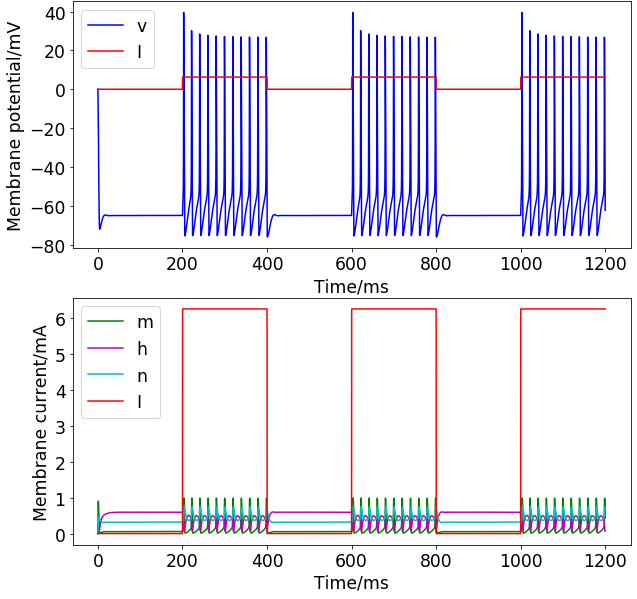
\includegraphics[width=\linewidth]{a6-26}
  \caption{6.26mA/nF}
  \label{sub:2a6-26}
  \end{subfigure}
  \begin{subfigure}[t]{0.49\textwidth}
    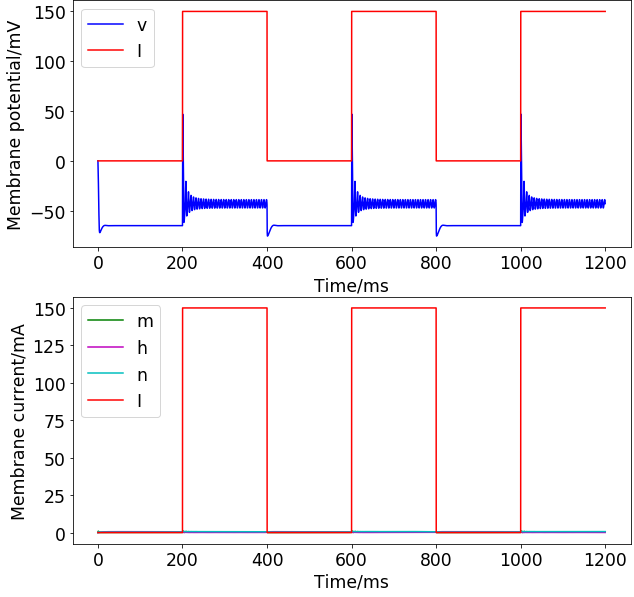
\includegraphics[width=\linewidth]{a150}
  \caption{150mA/nF}
  \label{sub:2a150}
  \end{subfigure}
  \caption{Example responses to 200ms pulse, 400ms period for different applied currents}
  \label{fig:2ae}
\end{figure}


%------------------------------------------------
\twocolumn
\subsection{ Variable period}
\begin{figure}[h]
  \centering
  \begin{subfigure}[t]{0.5\textwidth}
    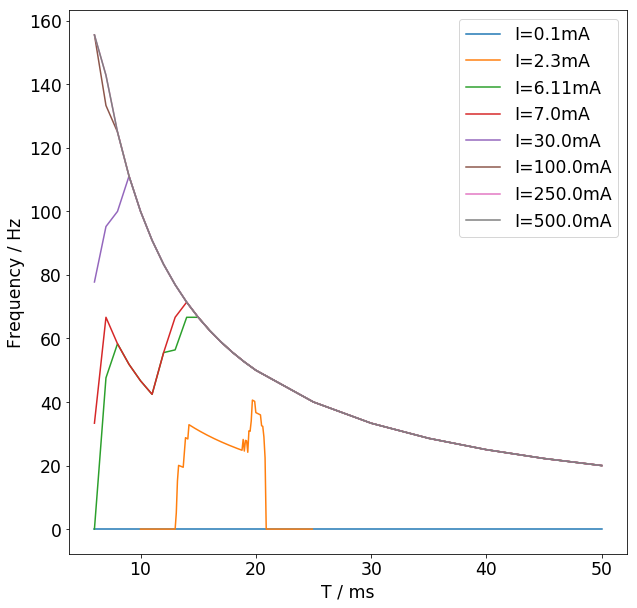
\includegraphics[width=\linewidth]{2aa}
  \caption{Spike frequency}
  \label{sub:2af}
  \end{subfigure}
  \begin{subfigure}[t]{0.5\textwidth}
    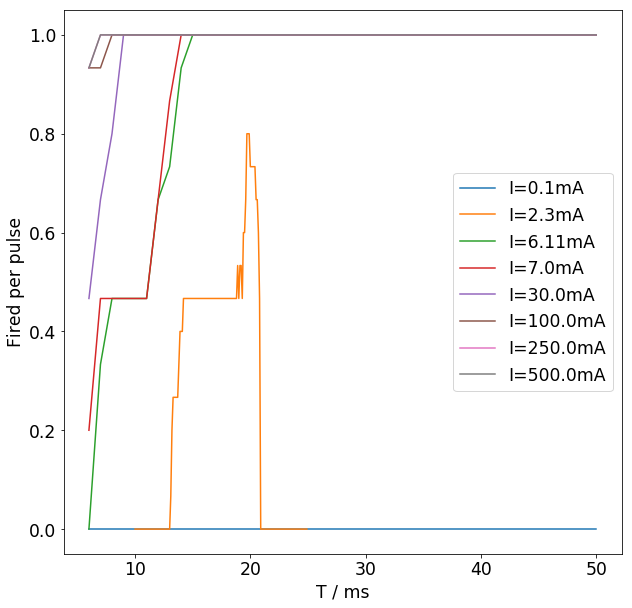
\includegraphics[width=\linewidth]{2ab}
  \caption{Spikes per pulse}
  \label{sub:2ap}
  \end{subfigure}
  \caption{Neuron response to 5ms pulse with variable period}
  \label{fig:2b}
\end{figure}
The input was next changed to allow for variation in period. A pulse length of 5ms was used with periods from 6ms to 50ms tested with different amplitudes, 15 periods were simulated. Figure \ref{sub:2af} shows the spiking frequency of the investigations. As the frequency was dependant on a variable(T) it was clearer to instead compare spikes per pulse as in figure \ref{sub:2ap}. The test inputs were chosen to be at points of interest from the previous experiment.
\newline
 At an input of 2.3mA/nF sharp threshold was once again observed at periods of 13.5ms and 21ms. Figures \ref{sub:2b23-13}-\ref{sub:2b23-20} show example plots of this behaviour. The spike count never reached an average of one spike per peak for this input, this shows that there is some instability in the dynamics which cause some pulses to not initiate a spike as in figure \ref{sub:2b23-20}. At periods of 18.7ms this instability was very variable and caused the noisy point point on figure \ref{sub:2ap}.
\newline
For a small input of 0.1mA/nF no spiking response was seen as with a constant pulse. Inputs 6.11mA/nF and 7mA/nF were chosen as this was the threshold for continuous firing for a constant pulse. Figure \ref{sub:2ap} shows that the spiking behaviour of both was very similar, and initially started at no spiking or firing at 1 in 5 pulses and increased to one spike per pulse with a 14ms period. Alternate pulse spiking was observed before reaching consistent spiking. Figures \ref{sub:2b7-7}-\ref{sub:2b7-50} show this behaviour. Additional combinations of spikes were observed at 6.11mA/nF where every fourth pulse resulted in no response at a 13ms period, this is shown in figure \ref{sub:2b61-13}. These extra periodic behaviours indicate more complicated limit cycles present in the system.
\newline
As the input increased a smaller period was required to reach consistent firing on each pulse. This indicated that the input has an effect of the recovery time of the system.






\onecolumn

\begin{figure}[h]
  \centering
  \begin{subfigure}[t]{0.49\textwidth}
    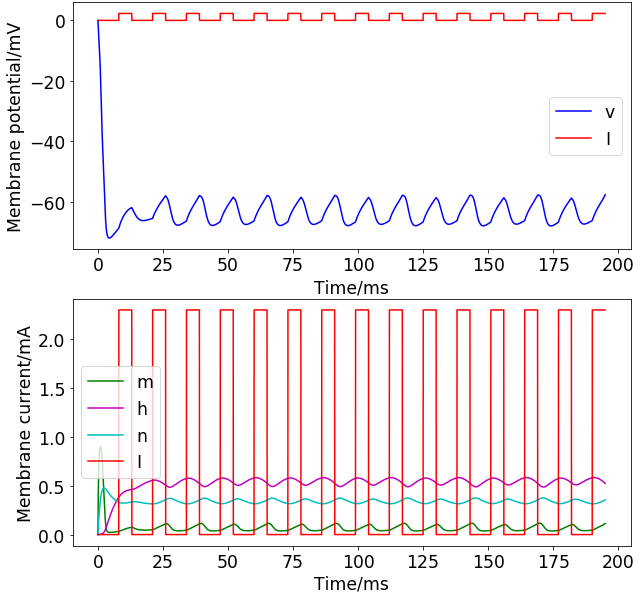
\includegraphics[width=\linewidth]{23-13}
  \caption{I=2.3mA/nF, T=13ms}
  \label{sub:2b23-13}
  \end{subfigure}
  \begin{subfigure}[t]{0.49\textwidth}
    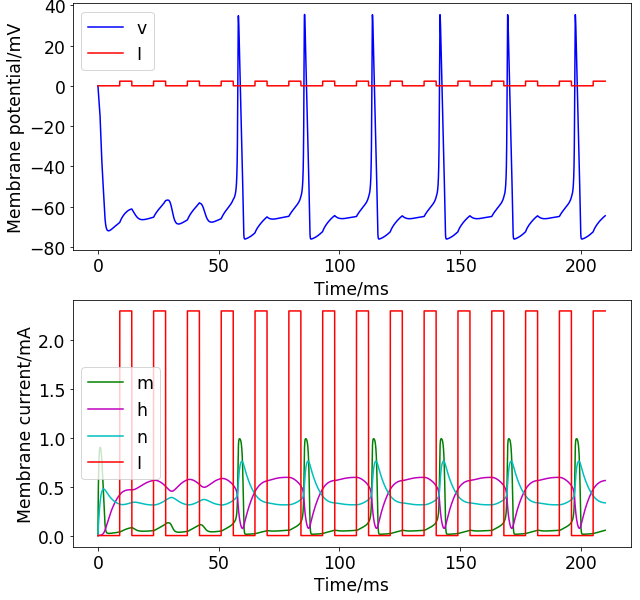
\includegraphics[width=\linewidth]{23-14}
  \caption{I=2.3mA/nF, T=14ms}
  \label{sub:2b23-14}
  \end{subfigure}
\newline
  \begin{subfigure}[t]{0.49\textwidth}
    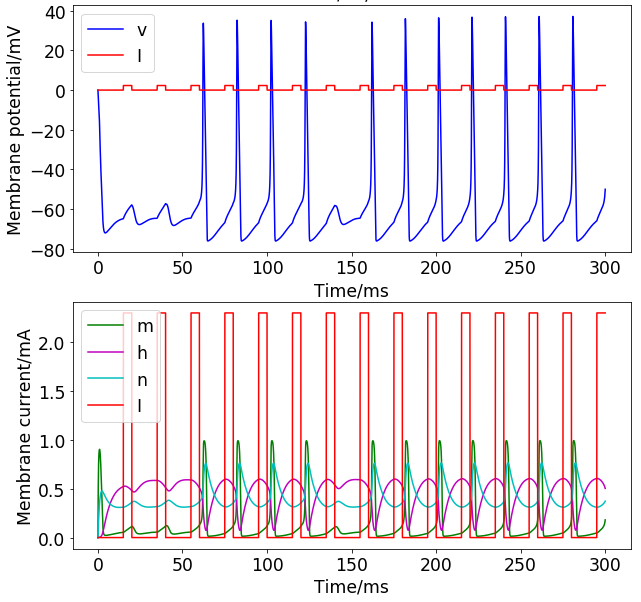
\includegraphics[width=\linewidth]{23-20}
  \caption{I=2.3mA/nF, T=20ms}
  \label{sub:2b23-20}
  \end{subfigure}
  \begin{subfigure}[t]{0.49\textwidth}
    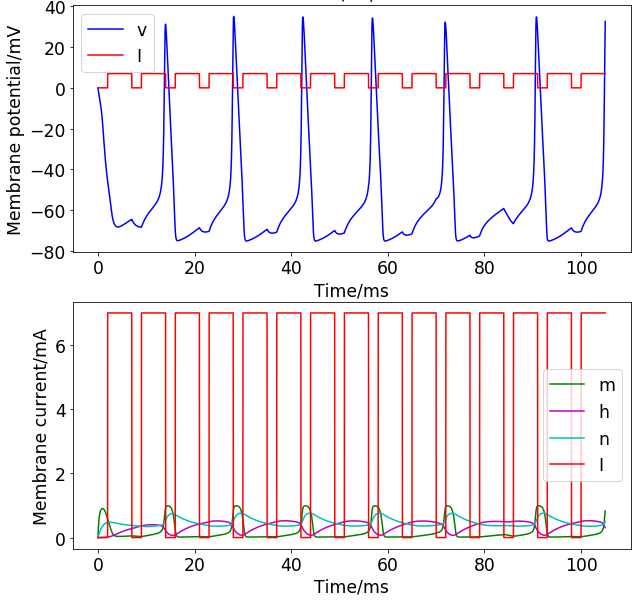
\includegraphics[width=\linewidth]{7-7}
  \caption{I=7mA/nF, T=7ms}
  \label{sub:2b7-7}
  \end{subfigure}
\newline
\begin{subfigure}[t]{0.49\textwidth}
    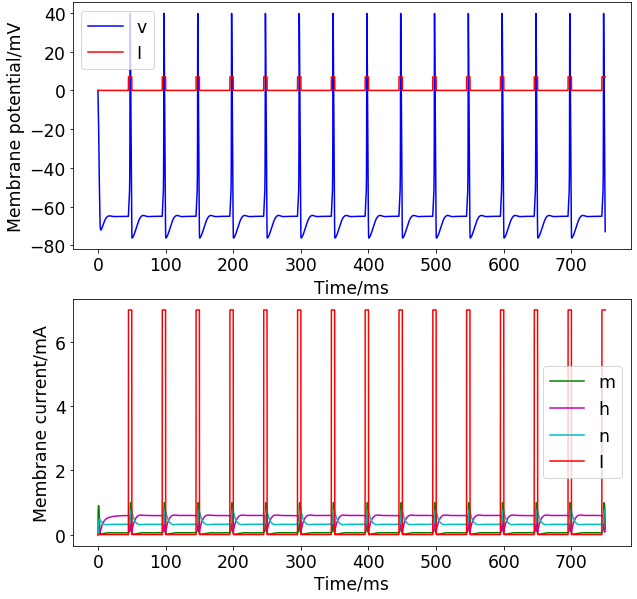
\includegraphics[width=\linewidth]{7-50}
  \caption{I=7mA/nF, T=50ms}
  \label{sub:2b7-50}
  \end{subfigure}
  \begin{subfigure}[t]{0.49\textwidth}
    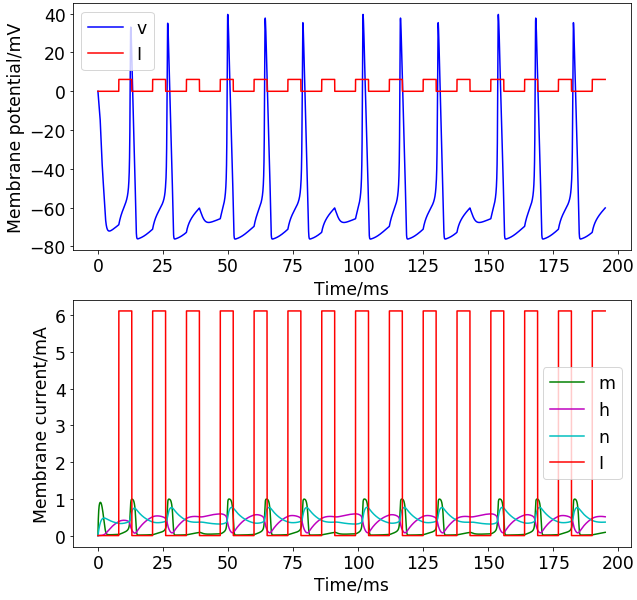
\includegraphics[width=\linewidth]{61-13}
  \caption{I=6.1mA/nF, T=13ms}
  \label{sub:2b61-13}
  \end{subfigure}
  \caption{Example responses for various periods(T) and applied currents(I) for a 5ms pulse}
  \label{fig:2be}
\end{figure}
%------------------------------------------------
\twocolumn
\subsection{ Variable pulse}

\begin{figure}[h]
  \centering
  \begin{subfigure}[t]{0.5\textwidth}
    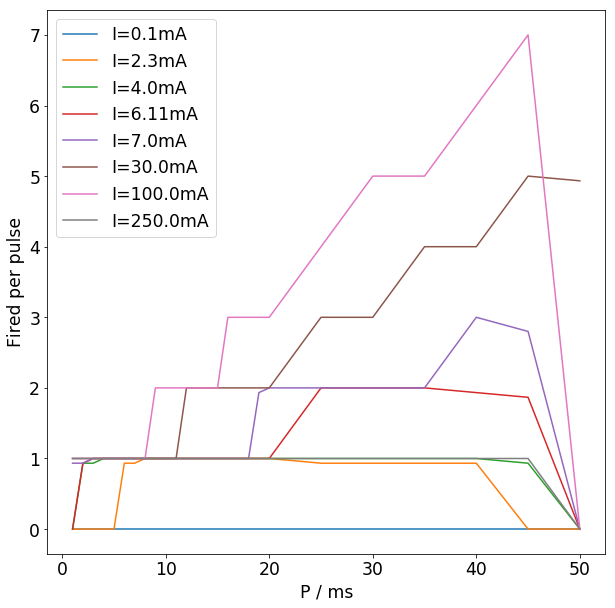
\includegraphics[width=\linewidth]{pf}
  \caption{}
  \label{sub:2cf}
  \end{subfigure}
  \begin{subfigure}[t]{0.5\textwidth}
    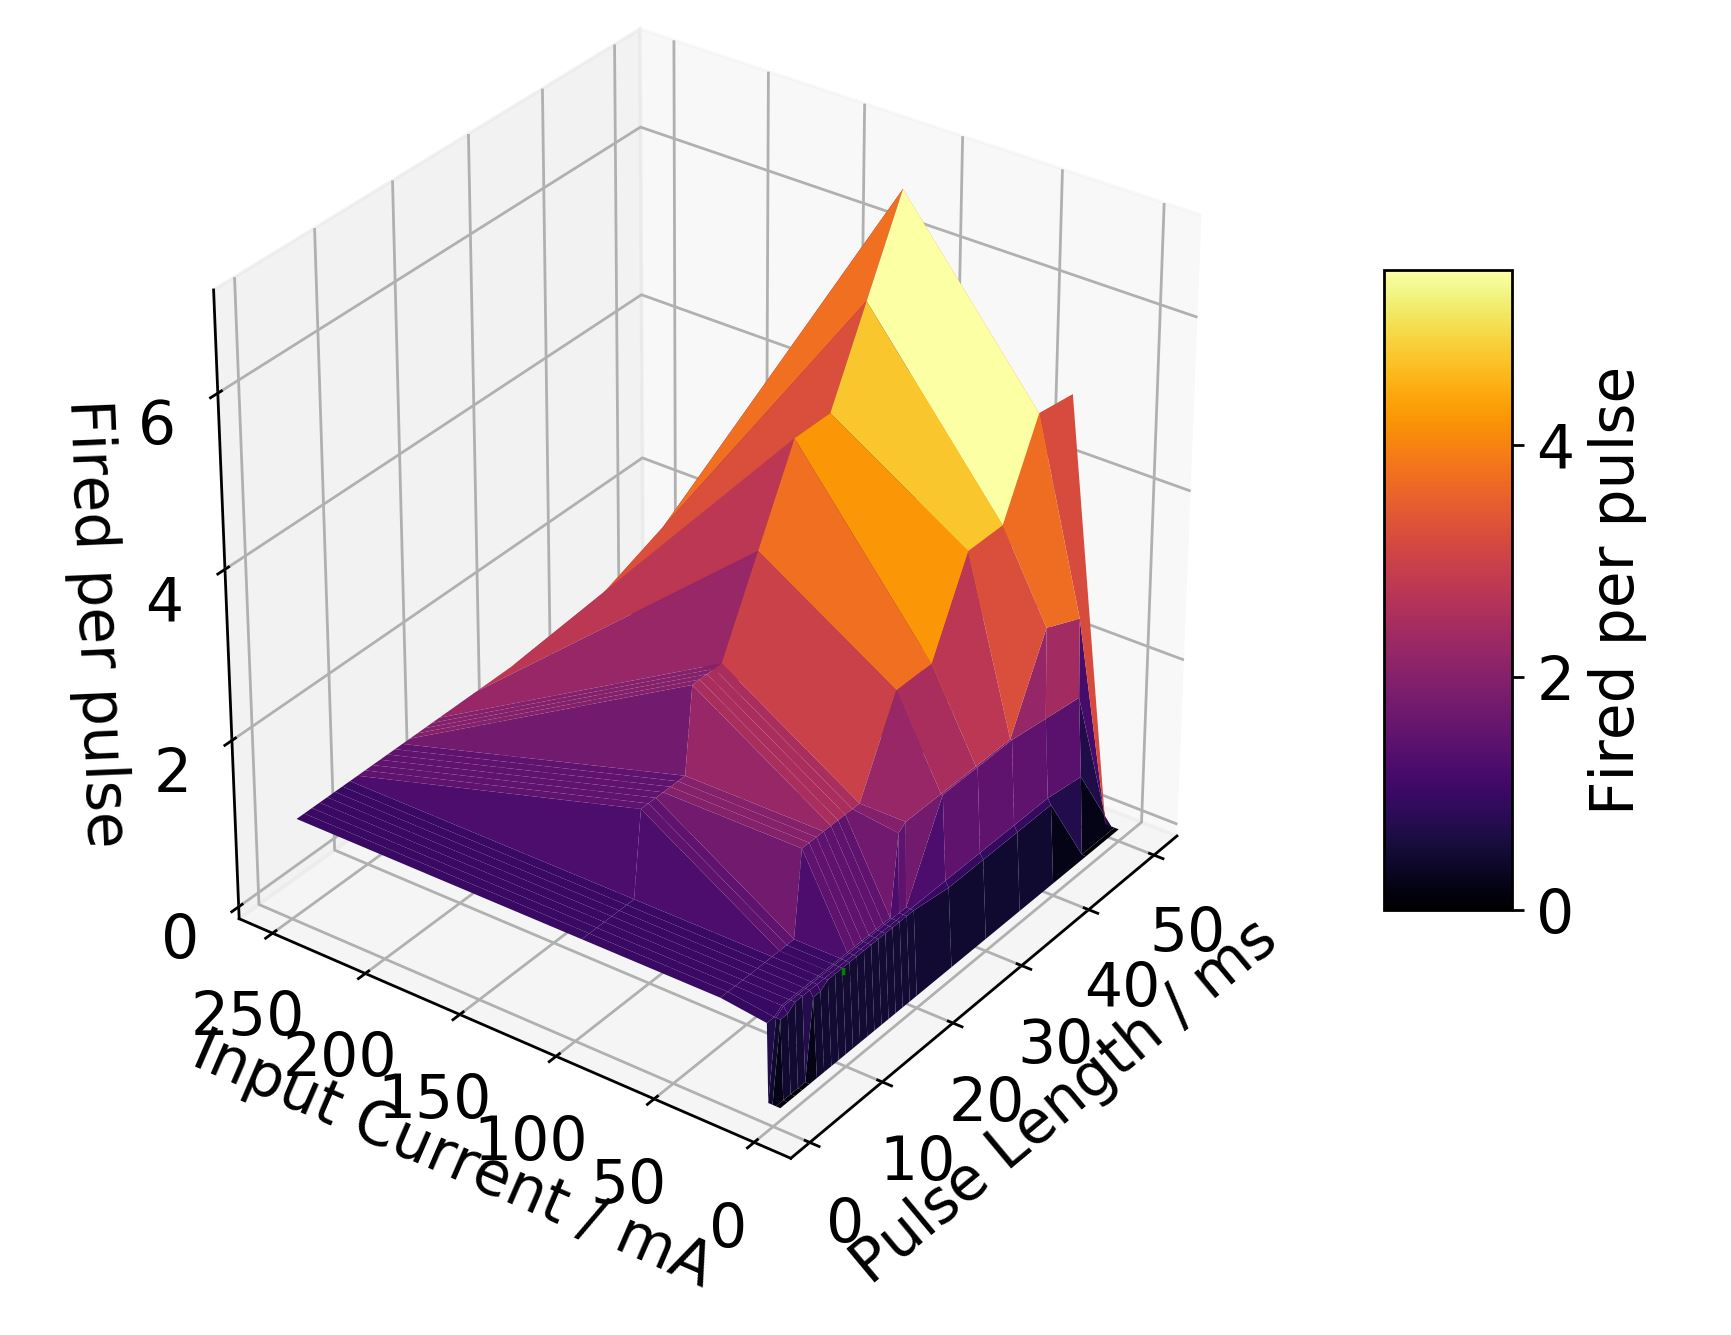
\includegraphics[width=\linewidth]{p3d}
  \caption{Surface plot}
  \label{sub:2c3d}
  \end{subfigure}
  \caption{Response when period was fixed to T=50ms}
  \label{fig:2c}
\end{figure}
A variable pulse length was investigated next, the period was fixed at 50ms and different currents were once again tested. Figure \ref{fig:2c} shows the counts per pulse achieved in this investigation. A complex surface is observed in figure \ref{sub:2c3d} showing peak response doesn't occur at maximum pulse length or current. This surface would include additional thresholds between currents if more simulations had been run. All responses decreased when a continuous input was applied, except at 30mA/nF. With this input and 50ms pulse length continuous firing was still occurring. This is seen in figure \ref{sub:2c30-50}, but looking at other inputs such as 100mA/nF as in figure \ref{sub:2c100-50} its clear that the input causes an oscillatory response of different amplitudes at other currents which weren't large enough to be counted as a spike in my tests. 
\newline
The spike position relative to pulse start time appears constant for a given input. Figures \ref{sub:2c7-1} and \ref{sub:2c7-45} show that a spike occurs within 2ms of a a pulse for an input of 7mA/nF. Figures \ref{sub:2c23-6} and \ref{sub:2c23-17} show that a spike occurs within 6ms of a a pulse for an input of 2.3mA/nF. This is expected as the membrane currents depend on the potential, which in turn is affected by the input current. As membrane currents change the time constant of the system will also be effected. 

\begin{figure}[h]
  \centering
    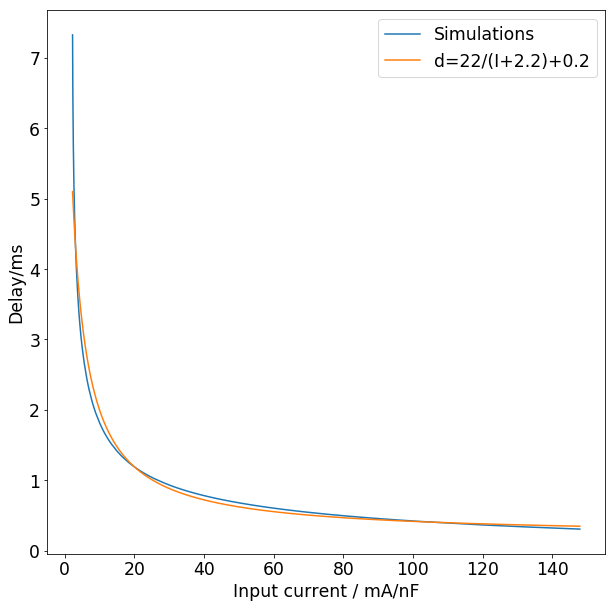
\includegraphics[width=\linewidth]{dm}
  \caption{Spike delay with 200ms pulse, 400ms period input}
  \label{fig:2del}
\end{figure}

Figure \ref{fig:2del} shows the delay in ms between pulse start and firing, for a 200ms pulse with 400ms period. The relationship observed can be approximately modelled by an equation of the form: delay = a/(I+b) +c. As this delay is predictable it can be useful in networks to add a desired delay especial at low currents where delay is highly sensitive.



\onecolumn

\begin{figure}[h]
  \centering
  \begin{subfigure}[t]{0.49\textwidth}
    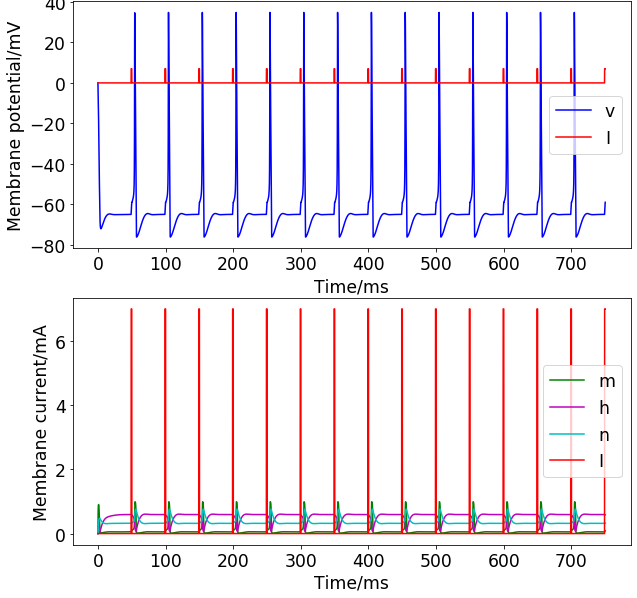
\includegraphics[width=\linewidth]{p7-1}
  \caption{I=7mA/nF, p=1ms}
  \label{sub:2c7-1}
  \end{subfigure}
  \begin{subfigure}[t]{0.49\textwidth}
    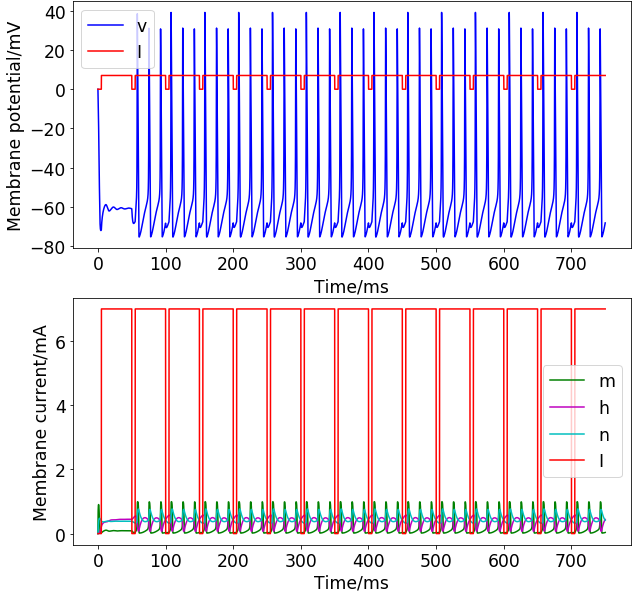
\includegraphics[width=\linewidth]{p7-45}
  \caption{I=7mA/nF, p=45ms}
  \label{sub:2c7-45}
  \end{subfigure}
\newline
  \begin{subfigure}[t]{0.49\textwidth}
    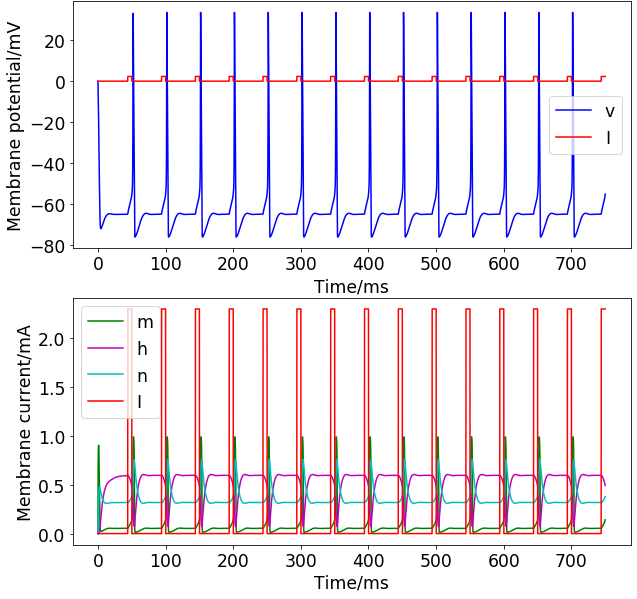
\includegraphics[width=\linewidth]{p23-6}
  \caption{I=2.3mA/nF, p=6ms}
  \label{sub:2c23-6}
  \end{subfigure}
  \begin{subfigure}[t]{0.49\textwidth}
    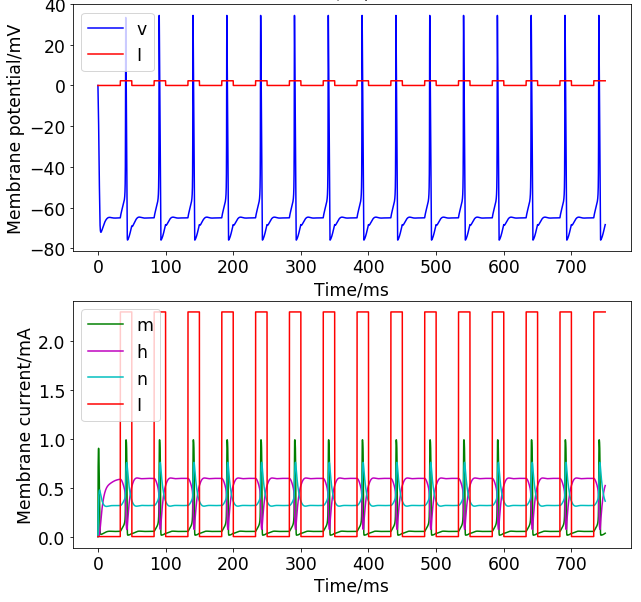
\includegraphics[width=\linewidth]{p23-17}
  \caption{I=2.3mA/nF, p=17ms}
  \label{sub:2c23-17}
  \end{subfigure}
\newline
\begin{subfigure}[t]{0.49\textwidth}
    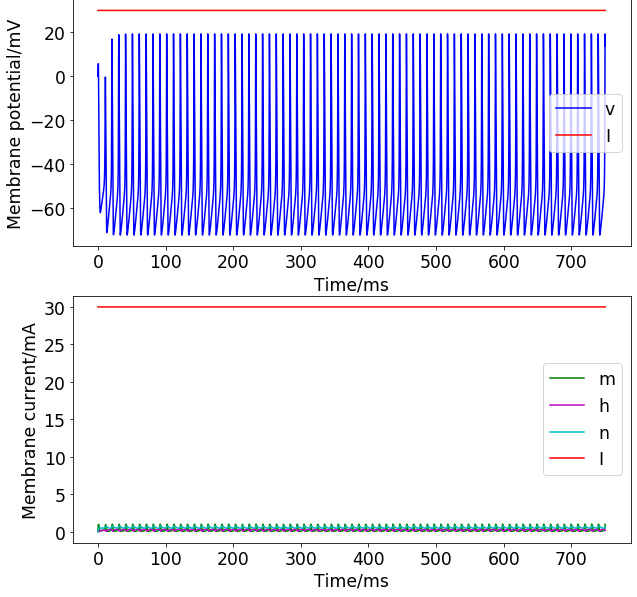
\includegraphics[width=\linewidth]{p30-50}
  \caption{I=30mA/nF, p=50ms}
  \label{sub:2c30-50}
  \end{subfigure}
  \begin{subfigure}[t]{0.49\textwidth}
    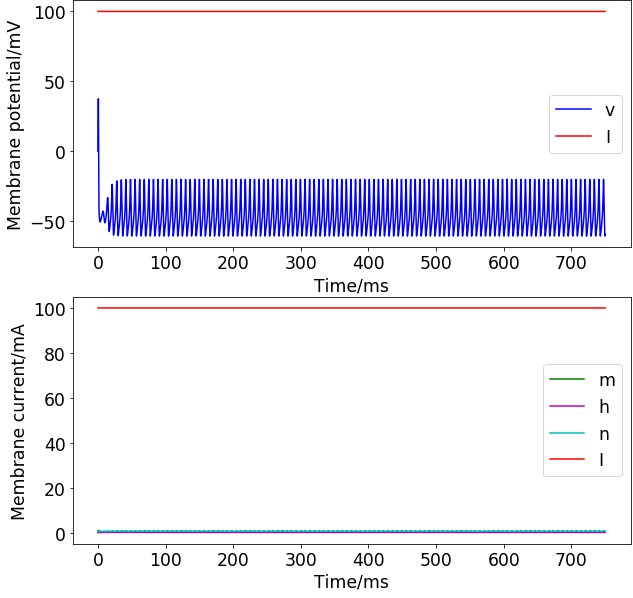
\includegraphics[width=\linewidth]{p100-50}
  \caption{I=100mA/nF, p=50ms}
  \label{sub:2c100-50}
  \end{subfigure}
  \caption{Example responses to different pulse lengths with a 50ms period}
  \label{fig:2ce}
\end{figure}

%------------------------------------------------
\twocolumn
\subsection{ Negative pulse}


\begin{figure}[h]
  \centering
    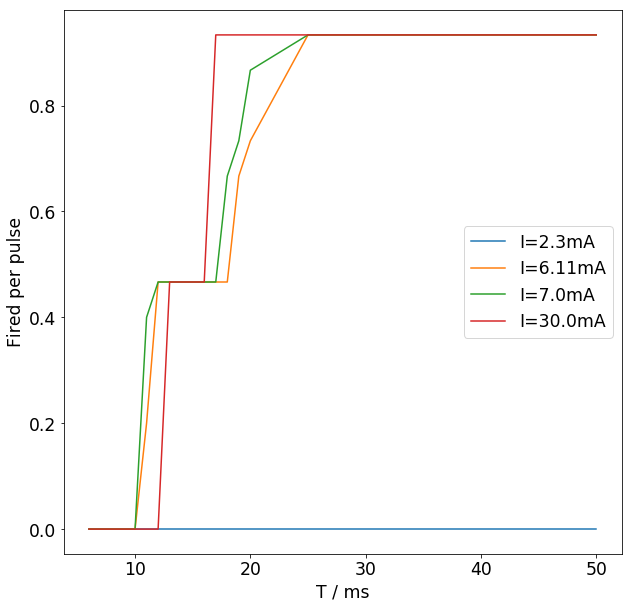
\includegraphics[width=\linewidth]{neg}
  \caption{Neuron response to negative current input}
  \label{fig:2d}
\end{figure}



Negative current inputs were investigated, it was found that interesting spiking behaviour and oscillatory responses were still possible at low negative currents. When the current got too large the membrane potential increased exponentially and broke simulations. Figure \ref{fig:2d} shows the effect of period length on spiking when a 5ms pulse is applied. A rate of 1 spike per peak is incorrectly not observed as the positive spike would have occurred after simulation time for the final pulse as an extra delay was present with negative inputs.
\newline
 A similar behaviour was observed in inputs of -6.11mA/nF and -7mA/nF as in figure \ref{sub:2ap}, however spiking occurred at a period of around 14ms compared to 5ms. No responses was observed to an input of -2.3mA/nF indicating the threshold was different for negative currents. Figure \ref{sub:2d23-50} shows this lack of spikes. For larger currents that worked in simulations such as -30mA/nF the spiking frequency was reduced to be similar to that of inputs around -6 to -7mA/nF. This input current also produced interesting oscillatory behaviour seen in figures \ref{sub:2d30-11}-\ref{sub:2d30-50}. Negative saw-wave oscillations, and negative spiking in addition to positive spikes are present in various frequencies. These responses could prove useful in situations where negative pulses are desired as well, creating a neuron that can act as inhibitory and excitatory. For example dopamine can be both a inhibitory and excitatory neurotransmitter.
\newline
A threshold of I= -2.8mA/nF was observed to initiate firing when using a 200ms pulse with 400ms period. Figure \ref{fig:2d2} shows this threshold and that a regular 1 spike per period is achieved for all currents that exceed this threshold.
\subsection{Conclusions}
\begin{itemize}
\item A sharp current threshold is observed to initiate continuous firing
\item Firing rate doesn't increase forever, another threshold is reached that reduced spikes down to 1 per pulse
\item The system resonates and fires 
\item Cyclic patterns of different orders are observed when using small pulse lengths, and negative currents
\item These patterns are the result of limit cycles present in the dynamics
\item Firing delay is a decreasing function of input current
\item Negative currents can cause both negative and positive spikes
\item Low potential oscillations can be produced with negative currents or when at currents that don't cause spikes
\end{itemize}
The wide variety of behaviours is useful in biology as it means neurons can be controlled with different inputs or modulators to produce the behaviour required in the current situation. This makes them very adaptable.
\newline
Resonators such as this model differ from more simplistic integrate and fire models as the firing rate is more likely when the input is at its resonant frequency, opposed to a higher frequency causing additional firing in integrators. This means that using the correct model for the biological system being studied can have great effect on the simulated responses. The simpler model while computationally faster will not include the complex behaviour present in resonators, so would be unsuitable in certain situations.

\onecolumn

\begin{figure}[h]
  \centering
  \begin{subfigure}[t]{0.49\textwidth}
    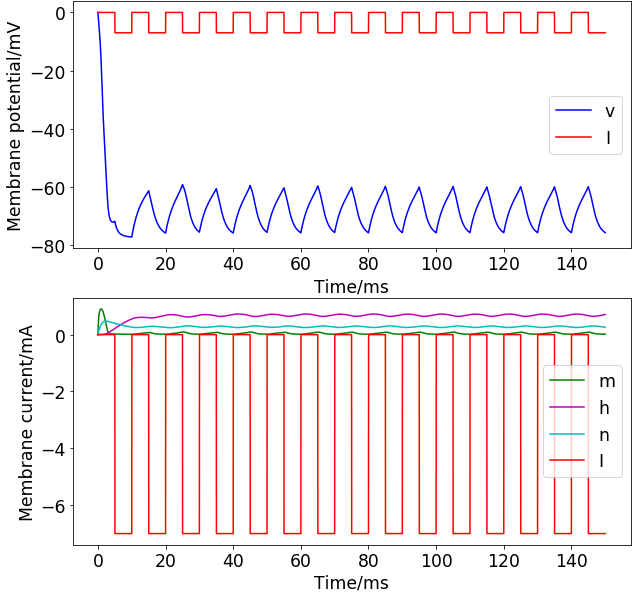
\includegraphics[width=\linewidth]{n7-10}
  \caption{I=-7mA/nF, T=10ms}
  \label{sub:2d7-10}
  \end{subfigure}
  \begin{subfigure}[t]{0.49\textwidth}
    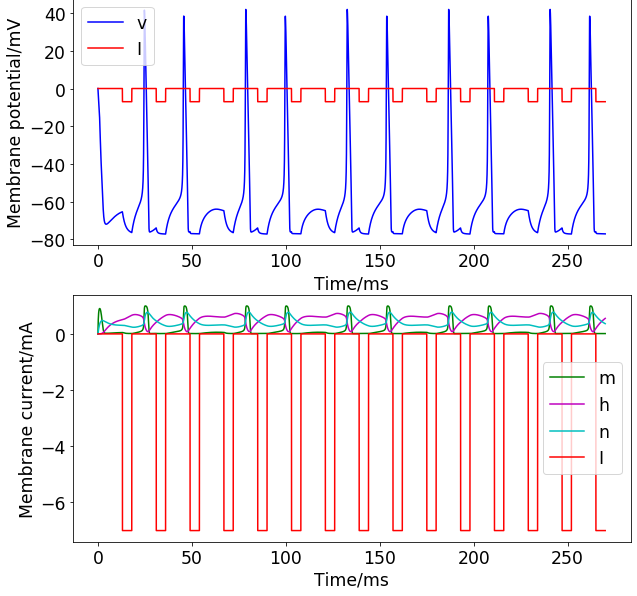
\includegraphics[width=\linewidth]{n7-18}
  \caption{I=-7mA/nF, T=18ms}
  \label{sub:2d7-18}
  \end{subfigure}
\newline
  \begin{subfigure}[t]{0.49\textwidth}
    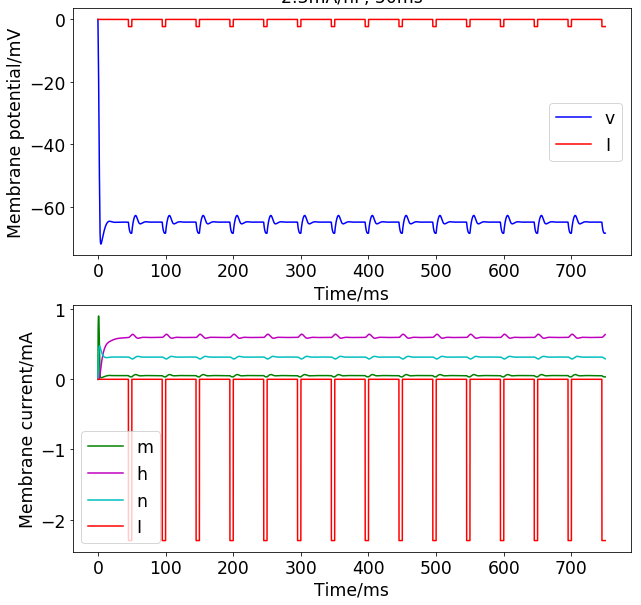
\includegraphics[width=\linewidth]{n23-50}
  \caption{I=-2.3mA/nF, T=50ms}
  \label{sub:2d23-50}
  \end{subfigure}
  \begin{subfigure}[t]{0.49\textwidth}
    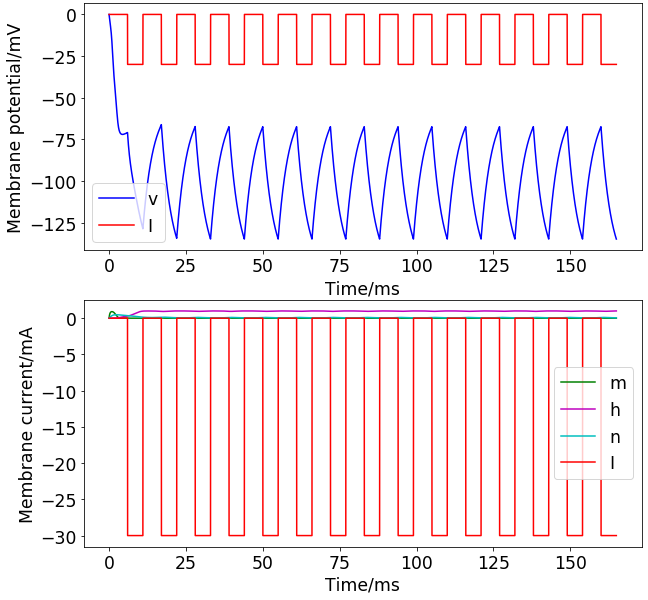
\includegraphics[width=\linewidth]{n30-11}
  \caption{I=-30mA/nF, T=11ms}
  \label{sub:2d30-11}
  \end{subfigure}
\newline
\begin{subfigure}[t]{0.49\textwidth}
    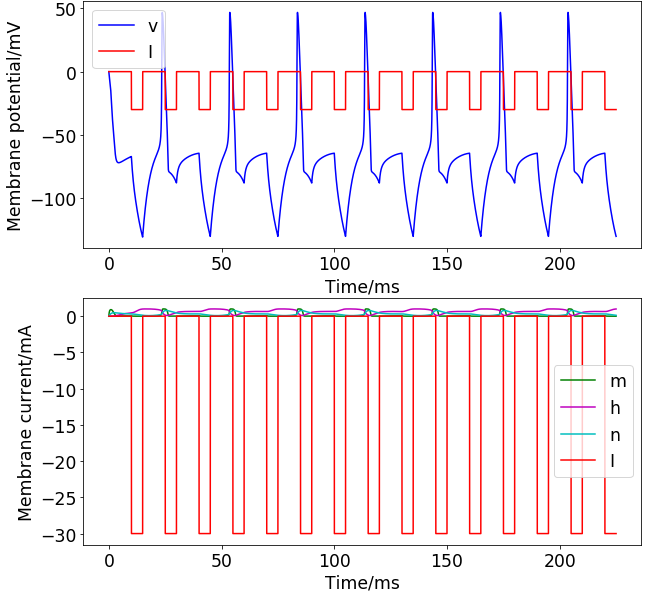
\includegraphics[width=\linewidth]{n30-15}
  \caption{I=-30mA/nF, T=15ms}
  \label{sub:2d30-15}
  \end{subfigure}
  \begin{subfigure}[t]{0.49\textwidth}
    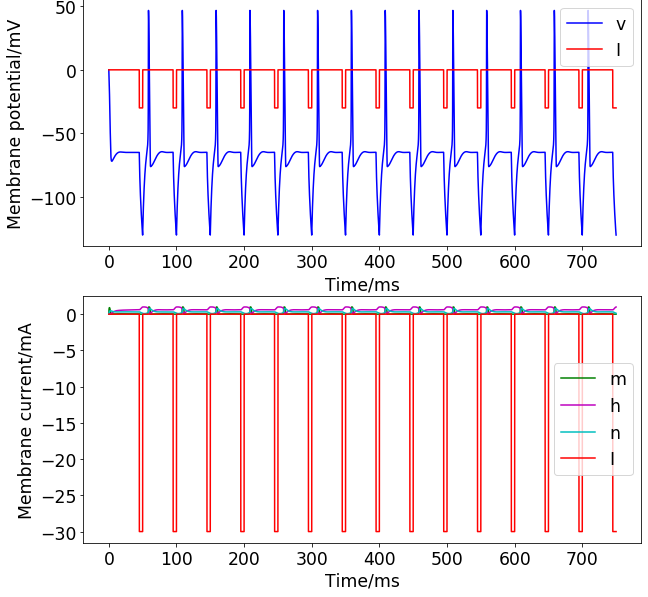
\includegraphics[width=\linewidth]{n30-50}
  \caption{I=-30mA/nF, T=50ms}
  \label{sub:2d30-50}
  \end{subfigure}
  \caption{Example responses to negative currents and different periods when p=5ms}
  \label{fig:2d}
\end{figure}
%------------------------------------------------
\twocolumn
\begin{figure}[h]
  \centering
    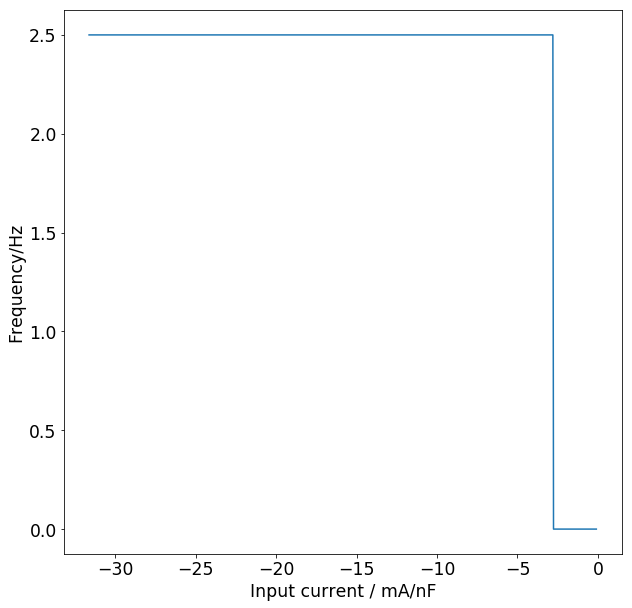
\includegraphics[width=\linewidth]{negr}
  \caption{Negative current input to regular pulse}
  \label{fig:2d2}
\end{figure}

%------------------------------------------------

%----------------------------------------------------------------------------------------

%------------------------------------------------
\end{document}
